\documentclass[
	ngerman,
	ruledheaders=section,
	class=report,
	thesis={type=Dokumentation},
	ignore-missing-data=true,
	accentcolor=9c,
	custommargins=false,
	marginpar=false,
	parskip=half-,
	fontsize=11pt,
]{tudapub}

% compatibility with older pdflatex versions
\usepackage{iftex}
\ifPDFTeX
	\usepackage[utf8]{inputenc}
\fi

% language packages
\usepackage[english, main=ngerman]{babel}
\usepackage[autostyle]{csquotes}

% tables
\usepackage{tabularx}
\usepackage{booktabs}

% mathematics
\usepackage{mathtools}
\usepackage{amssymb}
\usepackage{siunitx}
\sisetup{locale=DE}

% further packages
\usepackage[skip=10pt]{caption}
\usepackage{graphics,graphicx}
\usepackage[sf, SF]{subfigure}
\usepackage{listings}
\lstset{numbers=left, 
		numberstyle=\tiny, 
		numbersep=5pt, 
		backgroundcolor=\color{lightgray}, 
		xleftmargin=10pt, 
		showstringspaces=false, 
		tabsize=4}
\usepackage{epstopdf}
\usepackage{float}

% custom commands
\let\file\texttt
\let\code\texttt
\let\tbs\textbackslash
\let\pck\textsf
\let\cls\textsf
\newcommand{\mr}[1]{\mathrm{#1}}
\def\code#1{\texttt{#1}}

% start document
\setlength\intextsep{22pt}
\begin{document}

\Metadata{
	title=1. Hausübung - OpenCL,
	author=Leon Bohmann, Jonathan Stollberg
}

\title{1. Hausübung - OpenCL}
\author[]{Leon Bohmann (2493657) und Jonathan Stollberg (247775)}
\submissiondate{\today}

\maketitle
\tableofcontents

\chapter{Einführung}
In dieser Hausübung ging es darum die Berechnung eines Matrix-Vektor-Produkts gemäß
\begin{align*}
	c_{i} = A_{ij}b_{j}
\end{align*}
in der Programmiersprache \textit{Java} zu implementieren. Dabei soll die Matrix $\mathbf{A}$ stets quadratisch sein, d.h. $\mathbf{A} \in \mathbb{R}^{m\times m}$ und $\mathbf{b} \in \mathbb{R}^{m}$. Die Implementierung wurde sequentiell und parallel umgesetzt, wobei die Parallelisierung auf der GPU mittels der Schnittstelle \textit{OpenCL} erfolgt. %darauf geachtet wurde, dass das Programm sowohl auf der CPU mittels Streams als auch auf der GPU mittels der Schnittstelle \textit{OpenCL} parallelisiert ist.

Das Programm kann mittels der Kommandozeile mit zwei optionalen (und untrennbaren) Argumenten aufgerufen werden. Das erste Argument repräsentiert dabei die Problemgröße $m$, das zweite Argument legt die \textit{local size} fest, die der \textit{OpenCL} Kernel anfragt. Wird die Berechnung ganz ohne Argumente aufgerufen, so wird die Berechnung für verschiedene vordefinierte $m$ und \textit{local sizes} ausgeführt:
\begin{lstlisting}[language=bash]
	$ java -jar HighPerformanceSimulation.jar
	$ java -jar HighPerformanceSimulation.jar 1000 10
\end{lstlisting}

Im Folgenden sollen nun kurz wichtige Aspekte der Implementierung erläutert und anschließend die Performance der sequentiellen und parallelen Berechnungen für verschiedene $m$ analysiert und beurteilt werden.

\chapter{Sequentieller Algorithmus}
Zu Beginn des Programmaufrufs wird ausgehend von $m$ eine Zufallsmatrix $\mathbf{A}$ sowie ein Zufallsvektor $\mathbf{b}$ generiert. Diese werden als eindimensionale short-Arrays gespeichert, sodass auf das Element $A_{ij}$ über Index $i\times m + j$ zugegriffen wird. Für $\mathbf{b}$ ist der Zugriff über Indizes trivial.

Nachdem das Ergebnis-Array $\mathbf{c}$ der Länge $m$ initialisiert wurde, lässt sich die sequentielle Matrix-Vektor-Multiplikation nun mit wenigen Zeilen Code analog zur Einstein'schen Summenkonvention mithilfe von for-Schleifen implementieren:
\begin{lstlisting}[language=java]
	short[] c = new short[m];
	for (int i = 0; i < m; i++) {
		for (int j = 0; j < m; j++) {
			c[i] += A[i*m + j]*b[j];
		}
	}
\end{lstlisting}
Selbstverständlich muss der Code noch in eine Klassenstruktur bzw. eine Methode eingebunden werden. Für Weitere Details zur Implementierung wird an dieser Stelle an den beiliegenden den Code in der Datei \textit{MatrixVector.java} verwiesen.

\chapter{Paralleler Algorithmus mittels OpenCL}

\chapter{Performance-Analyse}
Die Performance-Tests wurden auf dem Lichtenberg-Hochleistungsrechner der Technischen Universität Darmstadt durchgeführt. Zu diesem Zwecke wurde ein SLURM-Skript geschrieben, welches einen Rechenknoten mit einer GPU des Typs \textit{NVIDIA A100-PCIE-40GB} für die Parallelisierung sowie einer CPU und 30 GB Speicher anfordert. Damit wurden die Tests für $m \in \{10, 100, 500, 1000, 2000, 4000, 5200\}$ gerechnet. Die \textit{local\_work\_size} wurde dabei zunächst von \textit{OpenCL} selbst festgelegt, anschließend aber auch noch variiert. Um die Rechenzeit möglichst unverfälscht zu zu untersuchen, wurde der Warmup der \textit{OpenCL}-Parallelisierung in allen Messungen ignoriert.

Die getesteten Problemgrößen unterscheiden sich zu den in der Aufgabenstellung vorgegebenen $m$, da am 03.12.2022 ab ca. 19:00 Uhr die benötigten Rechenknoten auf dem Lichtenberg-Hochleistungsrechner mit folgender Fehlermeldung nicht mehr aufrufbar waren:
\begin{lstlisting}
	$ Nodes required for job are DOWN, DRAINED or reserved for jobs 
	$ in higher priority partitions
\end{lstlisting}
Daher mussten wir auf bereits zuvor durchgeführte Tests zurückgreifen, was wir an dieser Stelle entschuldigen wollen.

In Abb.~\ref{auto_lws} sind die Rechenzeit und der Speedup für die unterschiedlichen $m$ und eine von \textit{OpenCL} festgelegte \textit{local size} dargestellt. Es ist zu erkennen, dass die parallele Matrix-Vektor-Multiplikation insbesondere für sehr große $m$ mit wesentlich geringerem Zeitaufwand durchgeführt wird, als im sequentiellen Fall. Somit wird im Falle $m = 5200$ bereits ein Speedup $S_p \approx 38$ erreicht.
\begin{figure}[h!tb]
	\centering
	\subfigure[Rechenzeit.]{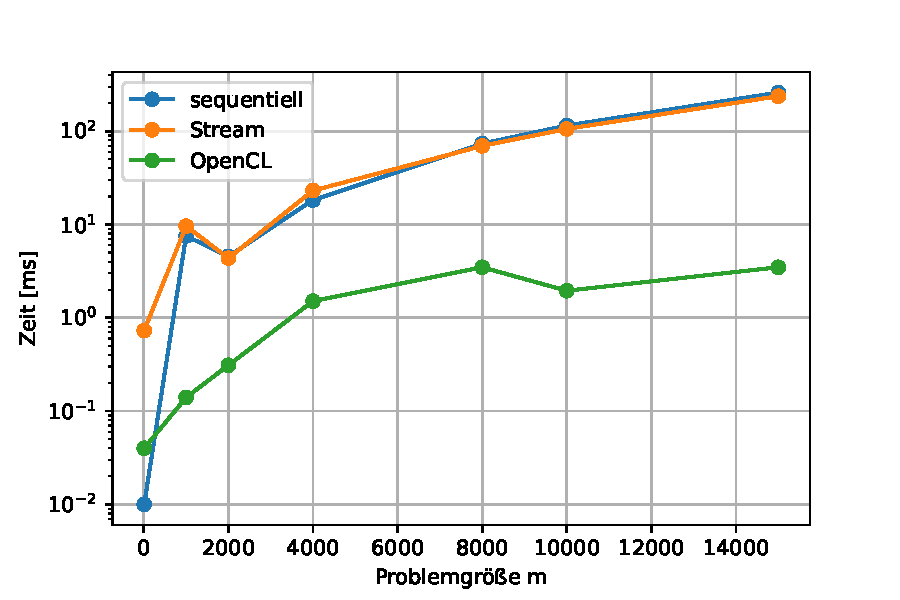
\includegraphics[width=14cm]{auto_lws.pdf}}\hspace{1cm}
	\subfigure[Speedup.]{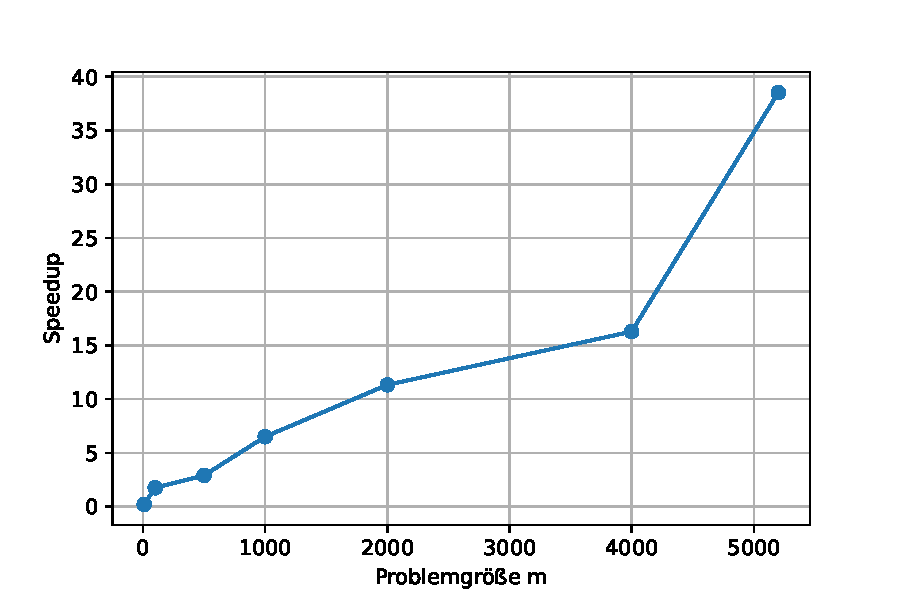
\includegraphics[width=14cm]{auto_speedup.pdf}}
	\caption{Matrix-Vektor-Multiplikation mit von \textit{OpenCL} automatisch festgelegter \textit{local\_work\_size}.}
	\label{auto_lws}
\end{figure}

\chapter{Fazit}

\end{document}
